\documentclass{article}

% Packages
\usepackage[utf8]{inputenc}

\usepackage{amsmath, bm}
\usepackage{graphicx}
\usepackage{amssymb}
\usepackage{float}
\usepackage{caption}
\usepackage{subcaption}
\usepackage{geometry}

\newgeometry{vmargin={1in}, hmargin={1in}}


\title{3A3 Compressor Lab Report}
\author{[Louis Pender]}
\date{\today}

\begin{document}

\maketitle

\section{Abstract}
% Provide a brief summary of the lab report, including the objective, methodology, and key findings.

\section{Introduction}

Two compressor setups were used in this experiment.
One with pure water, where the speed could be varied, and another using glycerine, a more viscous solution of 60\%
glycerine and 40\% water, where the compressor speed was fixed.
For the water setup, the flow rates were varied by screw valves at the inlet and outlet which were measured by pressure difference of a venturi flume.
The glycerine setup the flow rate was varied by a screw valve at outlet of the compressor, and was measured by timing a fixed volume of fluid.

\section{Theory}
% Describe the experimental setup, equipment used, and the steps followed during the experiment.

% Sketch the compressor rotor marking the inlet and exit flow directions and indicate which side
% of the blade is the suction surface and has the lowest average pressure and which is the pressure
% surface with the highest average pressure. Explain how you can determine which side is which.

% Sketch done on paper



\subsection{Non Dimensional Groups}

% Define a suitable non-dimensional cavitation number. Plot a graph of non-dimensional
% cavitation number against non-dimensional flow coefficient.

Two more non-dimensional groups are often used to characterise the flow in a compressor, the flow coefficient and the pressure rise coefficient.
These are defined as follows:
\begin{align}
    \text{Flow Coefficient} &= \frac{\dot{Q}}{ND^3} \label{eq:flow_coeff}\\
    \text{Pressure Coefficient} &= \frac{\Delta p}{\rho N^2 D^2} \label{eq:pressure_coeff}
\end{align}

The reynolds number at the outlet tips takes the standard form of:
\begin{equation}
    Re_{tip} = \frac{\rho ND^2}{\mu}
\end{equation}
Note: the factor of half from calculating the tip velocity is taken out to simplify the analysis.

Cavitation is caused by local pressure drops below that of the vapour pressure of the fluid, causing the fluid to vaporise.
The collapse of these bubbles can cause high pressure waves and damage to the impeller.
It is therefore important to predict the conditions under which cavitation is likely to occur.

It would also be expected that the further the local pressure drops below the vapour pressure, the more likely cavitation is to occur.
A non-dimensional number that could be used to predict cavitation would be the difference between the local pressure and the vapour pressure, divided by a dynamic pressure, given below.
\begin{equation}
    C_t = \frac{p - p_v}{\frac{1}{2}\rho v^2}
\end{equation}
At the inlet, where the pressure is predicted to be the lowest, $v = N \frac{D_1}{2}$
This gives a non-dimensional cavitation number of:
\begin{equation}
    C_t = 8\frac{p - p_v}{\rho (ND_1)^2}
\end{equation}
Cavitation was predicted to occur at the inlet of the compressor, where the velocity is highest and so pressure lowest.

To obtain the cavitation number $C_t$ at the inlet of the compressor, the pressure at the inlet of the compressor is required.
This was obtained by working backwards from the pressure at the discharge point being atmospheric.
The height of the reservoir discharge and outlet of the compressor is given as 570mm. The pressure loss from the
venturi flume is negligible and for the cases where the inlet valve was adjusted, there is no pressure drop through the fully open exit valve.
The pressure at the inlet of the compressor is therefore given by:
\begin{equation}
    p_1 =  P_a + \rho g h - \Delta p
\end{equation}
The vapour pressure of water rises with temperature as seen in figure \ref{fig:vapour_pressure_water} of the Appendix.
While the variation in temperature is small, the vapour pressure for each temperature datapoint is interpolated from this data, and is used in calculation for the cavitation number.

\subsection{Compressor Theory}

An attempt to determine the relationship between pressure rise and flow rate was made using the following theory.
For an isentropic compressor $Tds = 0 = dh_0 - vdp$ which relates the change specific stagnation enthalpy and static pressure as follows:
\begin{equation}
    w_s = \int_{p_1}^{p_2} vdp = \int_{p_1}^{p_2} \frac{dp}{\rho}
\end{equation}
Water can be taken as incompressible for the considered range of pressure, and so density is constant and can be taken out of the integral.
For a work input, $\dot{W}$ and flow rate $\dot{Q}$ the work done by a compressor at isentropic efficiency $\eta$ can be found as:
\begin{equation}
    \dot{W} = \frac{\rho \dot{Q} w_s}{\eta} = \frac{\dot{Q} \Delta p}{\eta} 
\end{equation}
This gives an inverse relationship between pressure rise and flow rate.
Rearanging and using definitions \ref{eq:flow_coeff} and \ref{eq:pressure_coeff} it can be shown that for constant compressor power, speed, and isentropic efficiency, the following relationship should hold:
\begin{equation}
    \text{Pressure Coefficient} \propto \frac{1}{\text{Flow Coefficient}} \label{eq:inverse_relationship}
\end{equation}
It is important to note that these assumptions are not strictly true, and the relationship is only used to make predictions about the behaviour of the compressor.

\subsection{Flow measurements}

For the water setup, the flow rate was measured using a venturi flume, which measures the pressure difference across a constriction in the flow.
\begin{equation}
    \dot{m} = C_f A_1 \sqrt{\frac{2\rho_w \Delta p}{1 - \left( \frac{A_1}{A_2} \right)^2}} \label{eq:venturi_flume}
\end{equation}
The calibrated discharge coefficient, and geomtry of the venturi flume were given in the form of a constant $a=0.193$ such that $\dot{m}=a \sqrt{\Delta p}$

For the glycerine setup, the flow rate was measured by timing a fixed volume of 15L of the solution.
The flow rate was therefore given by:
\begin{equation}
    \dot{Q} = \frac{V}{T}
\end{equation}
Which can easily be converted to mass flow rate using the known density $\rho_g$ of the glycerine solution.

% Velocity triangle on paper

% Using the mass flow rate and the impeller measurements, determine the radial velocity at the
% inlet to the blade at maximum flow condition, this is the starting value when valves are fully
% open. Non-dimensionalise your value by the blade speed.
The following analysis is based on the assumptions that:
\begin{itemize}
    \item The flow is incompressible.
    \item In the absolute frame, the inlet flow has only radial velocity.
\end{itemize} 

The radial inlet velocity can simply be calculated from continuity.
\begin{equation}
    v_1 = \frac{\dot{Q}}{\pi D_1 h} \label{eq:simple_radial_velocity}
\end{equation}
However, the impeller blades have an additional thickness $b$ which should be accounted for.
The angle of the blade to the circumferential direction is 30 degrees and so the circumferential width is $2b$.
The equation for the inlet velocity is then given by:
\begin{equation}
    v_1 = \frac{\dot{Q}}{(\pi D_1 - 2b N) h} \label{eq:radial_velocity}
\end{equation}
Where $N = 6$ blades for this compressor setup.

The relative velocity of the flow follows the leading edge and so at the inlet this makes an angle of $\chi_1$ to the radial direction.
This is shown in the velocity diagram in figure \ref{fig:vel_diagrams}.
From this, because the radial and tangential velocities are perpendicular,
the angle of the relative velocity to the radial direction is given by:
\begin{equation}
    \chi_1 = \arctan\left( \frac{u_1}{v_1} \right)
\end{equation}

The radial velocity $v_1$ can also be non dimensionalised by the inlet blade speed to give:
\begin{equation}
    \frac{v_1}{U_1} = \frac{2v_1}{N D_1}
\end{equation}


For the water setup at maximum flow condition, both inlet and outlet valves are fully open.
At the compressor speed of $298.97$ rad/s, $u_1 = 3.767 m/s$.
From equation \ref{eq:simple_radial_velocity}, $V_1 = 1.736 m/s$, $\chi_1 = 65.2^\circ$.
However, using equation \ref{eq:radial_velocity} gives $V_1 = 1.913 m/s$, $\chi_1 = 63.1^\circ$.
Accounting for the thickness of the blade has a significant effect on the radial velocity,
However, the angle of the relative velocity is not significantly affected.

These are close to the measured geometry of the impeller, and so the assumptions made are reasonable.

% Draw a velocity triangle for this situation and determine the relative velocity at the inlet to the
% rotor blade. 

\begin{figure}[H]
    \centering
    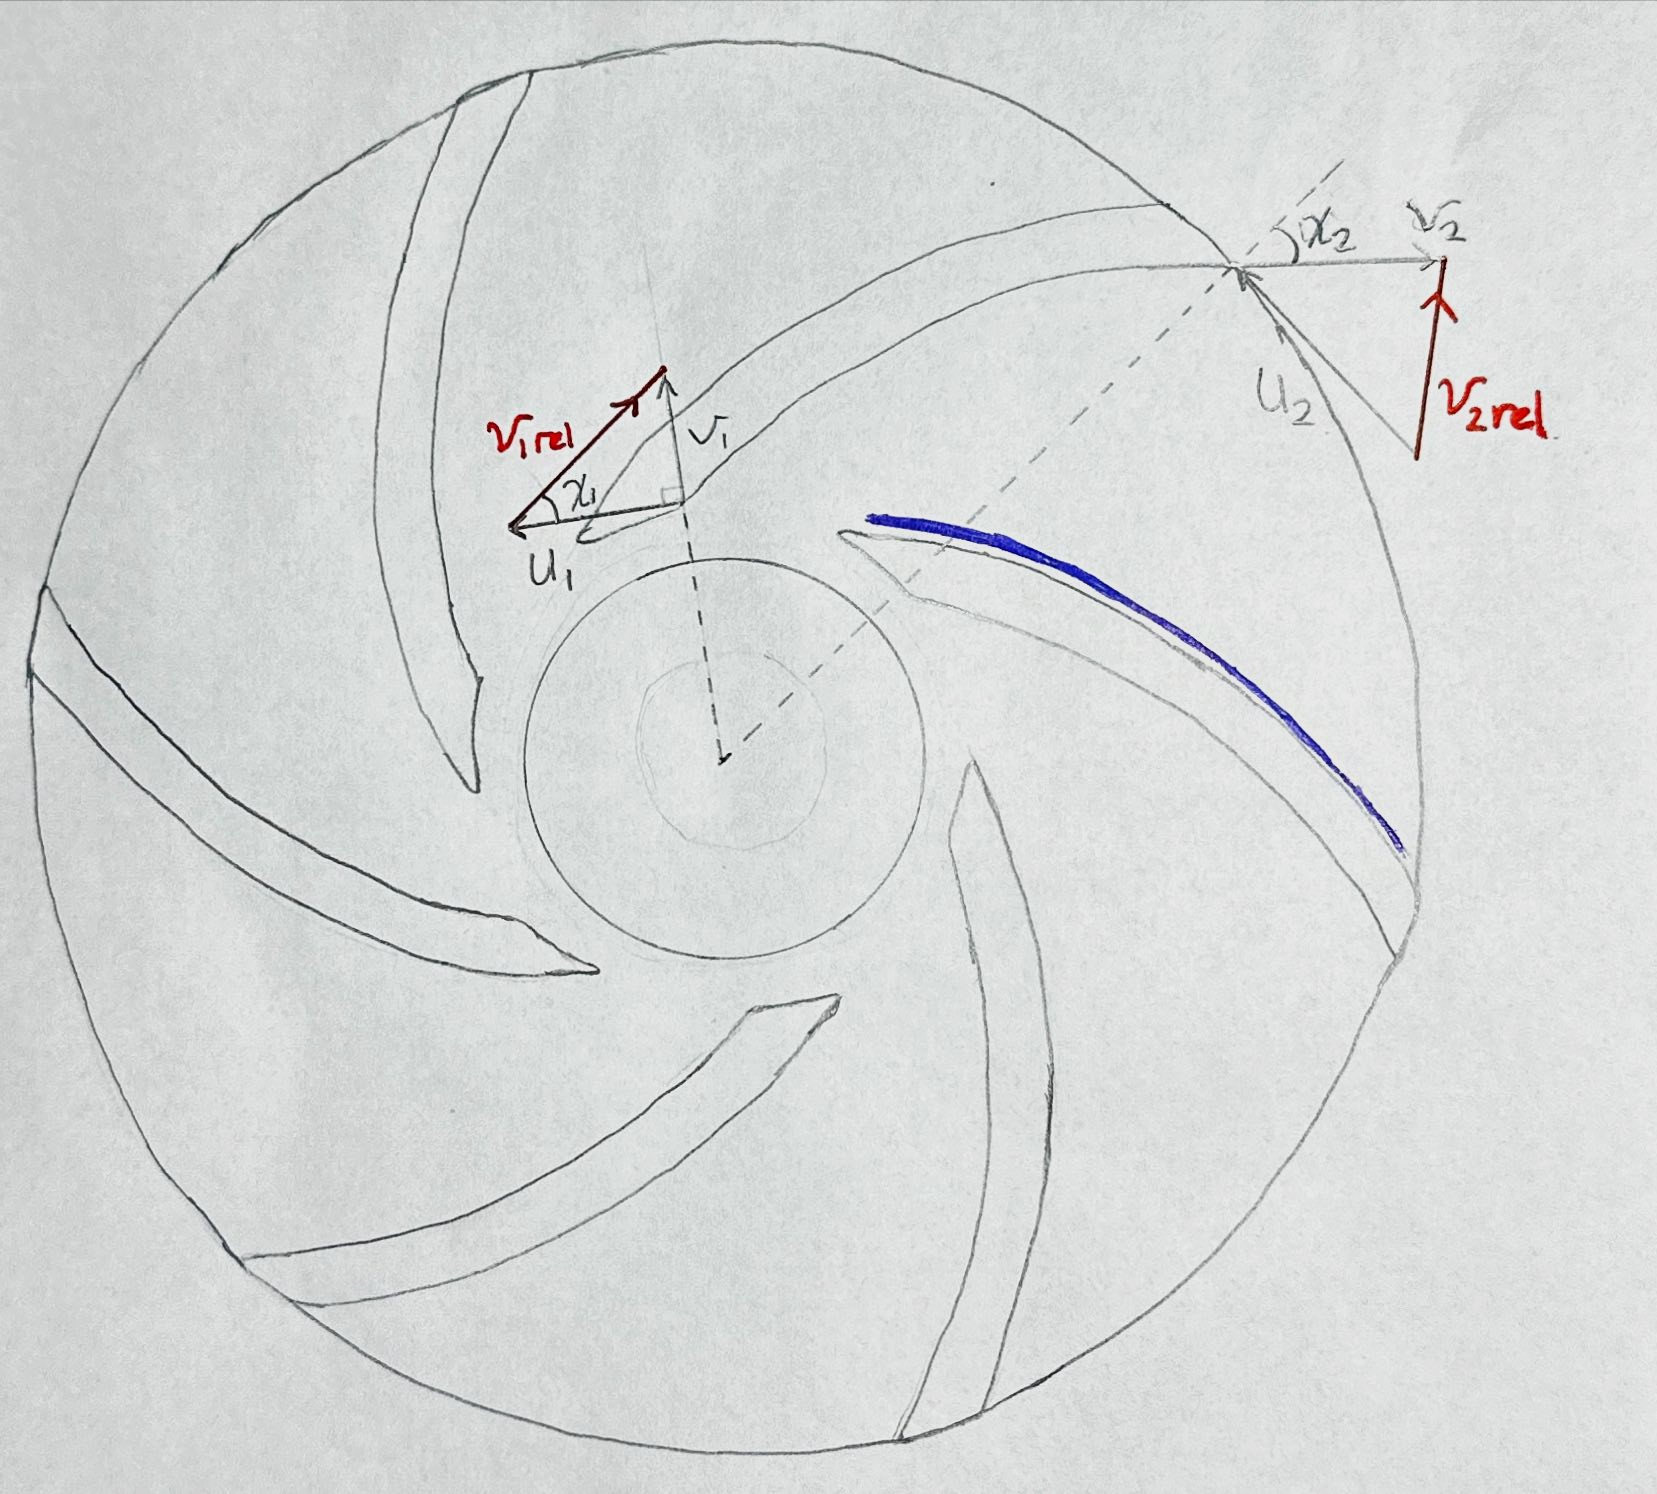
\includegraphics[width=0.6\textwidth]{velocity_diagrams.jpg}
    \caption{Compressor sketch and velocity diagrams. The high pressure surface is indicated by the red line, with the suction surface as the blue line.
    Note: Velocity triangles will have different scales.}
    \label{fig:vel_diagrams}
\end{figure}


% Use this velocity, the inlet diameter of the impeller and the kinematic viscosity of
% water to estimate the Reynolds number for the compressor. The magnitude of this Reynolds
% number will be comparable to values that you are familiar with for pipe flow

The reynolds number at the inlet of the compressor is given by:
\begin{equation}
    Re_{in} = \frac{\rho v_1 D_1}{\mu}
\end{equation}


\subsection{Viscosity measurements}
% viscosity theory.

The viscosity of water is well known at standard conditions, however the viscosity of the glycerine solution is not.
However, using thin film theory, the time taken for a fluid to travel a specific distance can be used to determine the viscosity of the fluid.

\begin{equation}
    \mu \propto \frac{T\rho}{L}
\end{equation}
    
Where $\mu$ is the dynamic viscosity, $T$ is the time taken for the fluid to travel a distance $L$, and $\rho$ is the density of the fluid.
This can be used to determine the ratio of dynamic viscosities
\section{Results}
% Present the data obtained from the experiment, including tables, graphs, and figures.

% Plot all the five measured pressure rise characteristics on a single graph. Ensure the graph is
% sufficiently large and has a true zero on both axes. The 5 curves are: 2x full speed and 2x half
% speed for the water circuit and 1x full speed for the glycerine circuit.

\subsection{Impeller Geometry}

\begin{figure}[H]
    \centering
    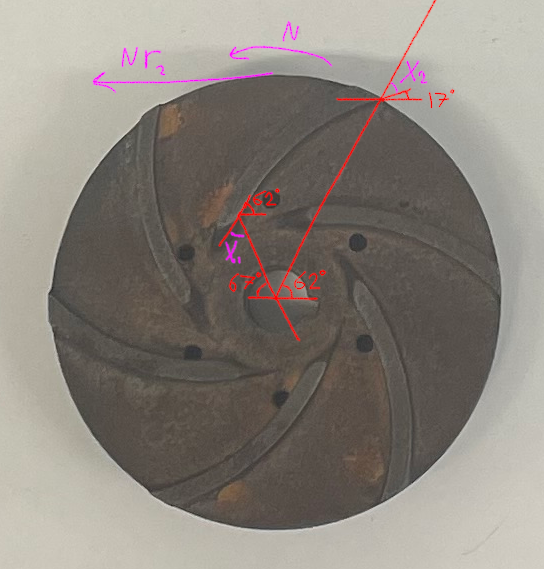
\includegraphics[width=0.6\textwidth]{impeller_annotations.png}
    \caption{Example image}
    \label{fig:impeller_annotations}
\end{figure}

And so angles for the leading edge of the impeller blades to the radial direction are given by:
\begin{alignat}{2}
    \chi_1 &= 180-73-36 &= 71^\circ \notag \\
    \chi_2 &= 8 + 36 &= 44^\circ \notag
\end{alignat}

These values are shown in the table below, along with additional inlet and outlet diameter measurements with callipers.

\begin{table}[H]
    \centering
    \begin{tabular}{|c|c|}
        \hline
        \textbf{Quantity} & \textbf{Value} \\
        \hline
        Inlet Diameter $D_1$ & 25.2 mm \\
        Outlet Diameter $D_2$ & 79.3 mm \\
        Blade Span $h$ & 6.40 mm \\
        Blade Width $b$ & 3.9 mm \\
        Inlet Blade Angle $\chi_1$ & $51^\circ$ \\
        Outlet Blade Angle $\chi_2$ & $45^\circ$ \\
        \hline
    \end{tabular}
    \caption{Impeller geometry measurements.}
    \label{tab:impeller_geometry}
\end{table}

The ambient pressure was measured as $754$ mmHg, corresponding to $100.56$ kPa.

\subsection{Viscosiy measurements}

At the ambient conditions the density of water is $998.2 kg/m^3$.
The density of the glycerine solution was known to be $1170 kg/m^3$.

\begin{table}[H]
    \centering
    \begin{tabular}{|c|c|c|}
        \hline
        \textbf{Length} $(m)$ & \textbf{Time} (s) & \textbf{Density} ($kg/m^3$) \\
        \hline
        10 & 40.35 & 998.2 \\
        2 & 102.01 & 1170 \\
        \hline
    \end{tabular}
    \caption{Time taken for 10mL of fluid to travel a specific length at $18.3^\circ C.$}
    \label{tab:viscosity}
\end{table}

The ratio of dynamic viscosities of the fluids is given by the ratio of time to length.

\subsection{Compressor Data}

\begin{figure}[H]
    \centering
    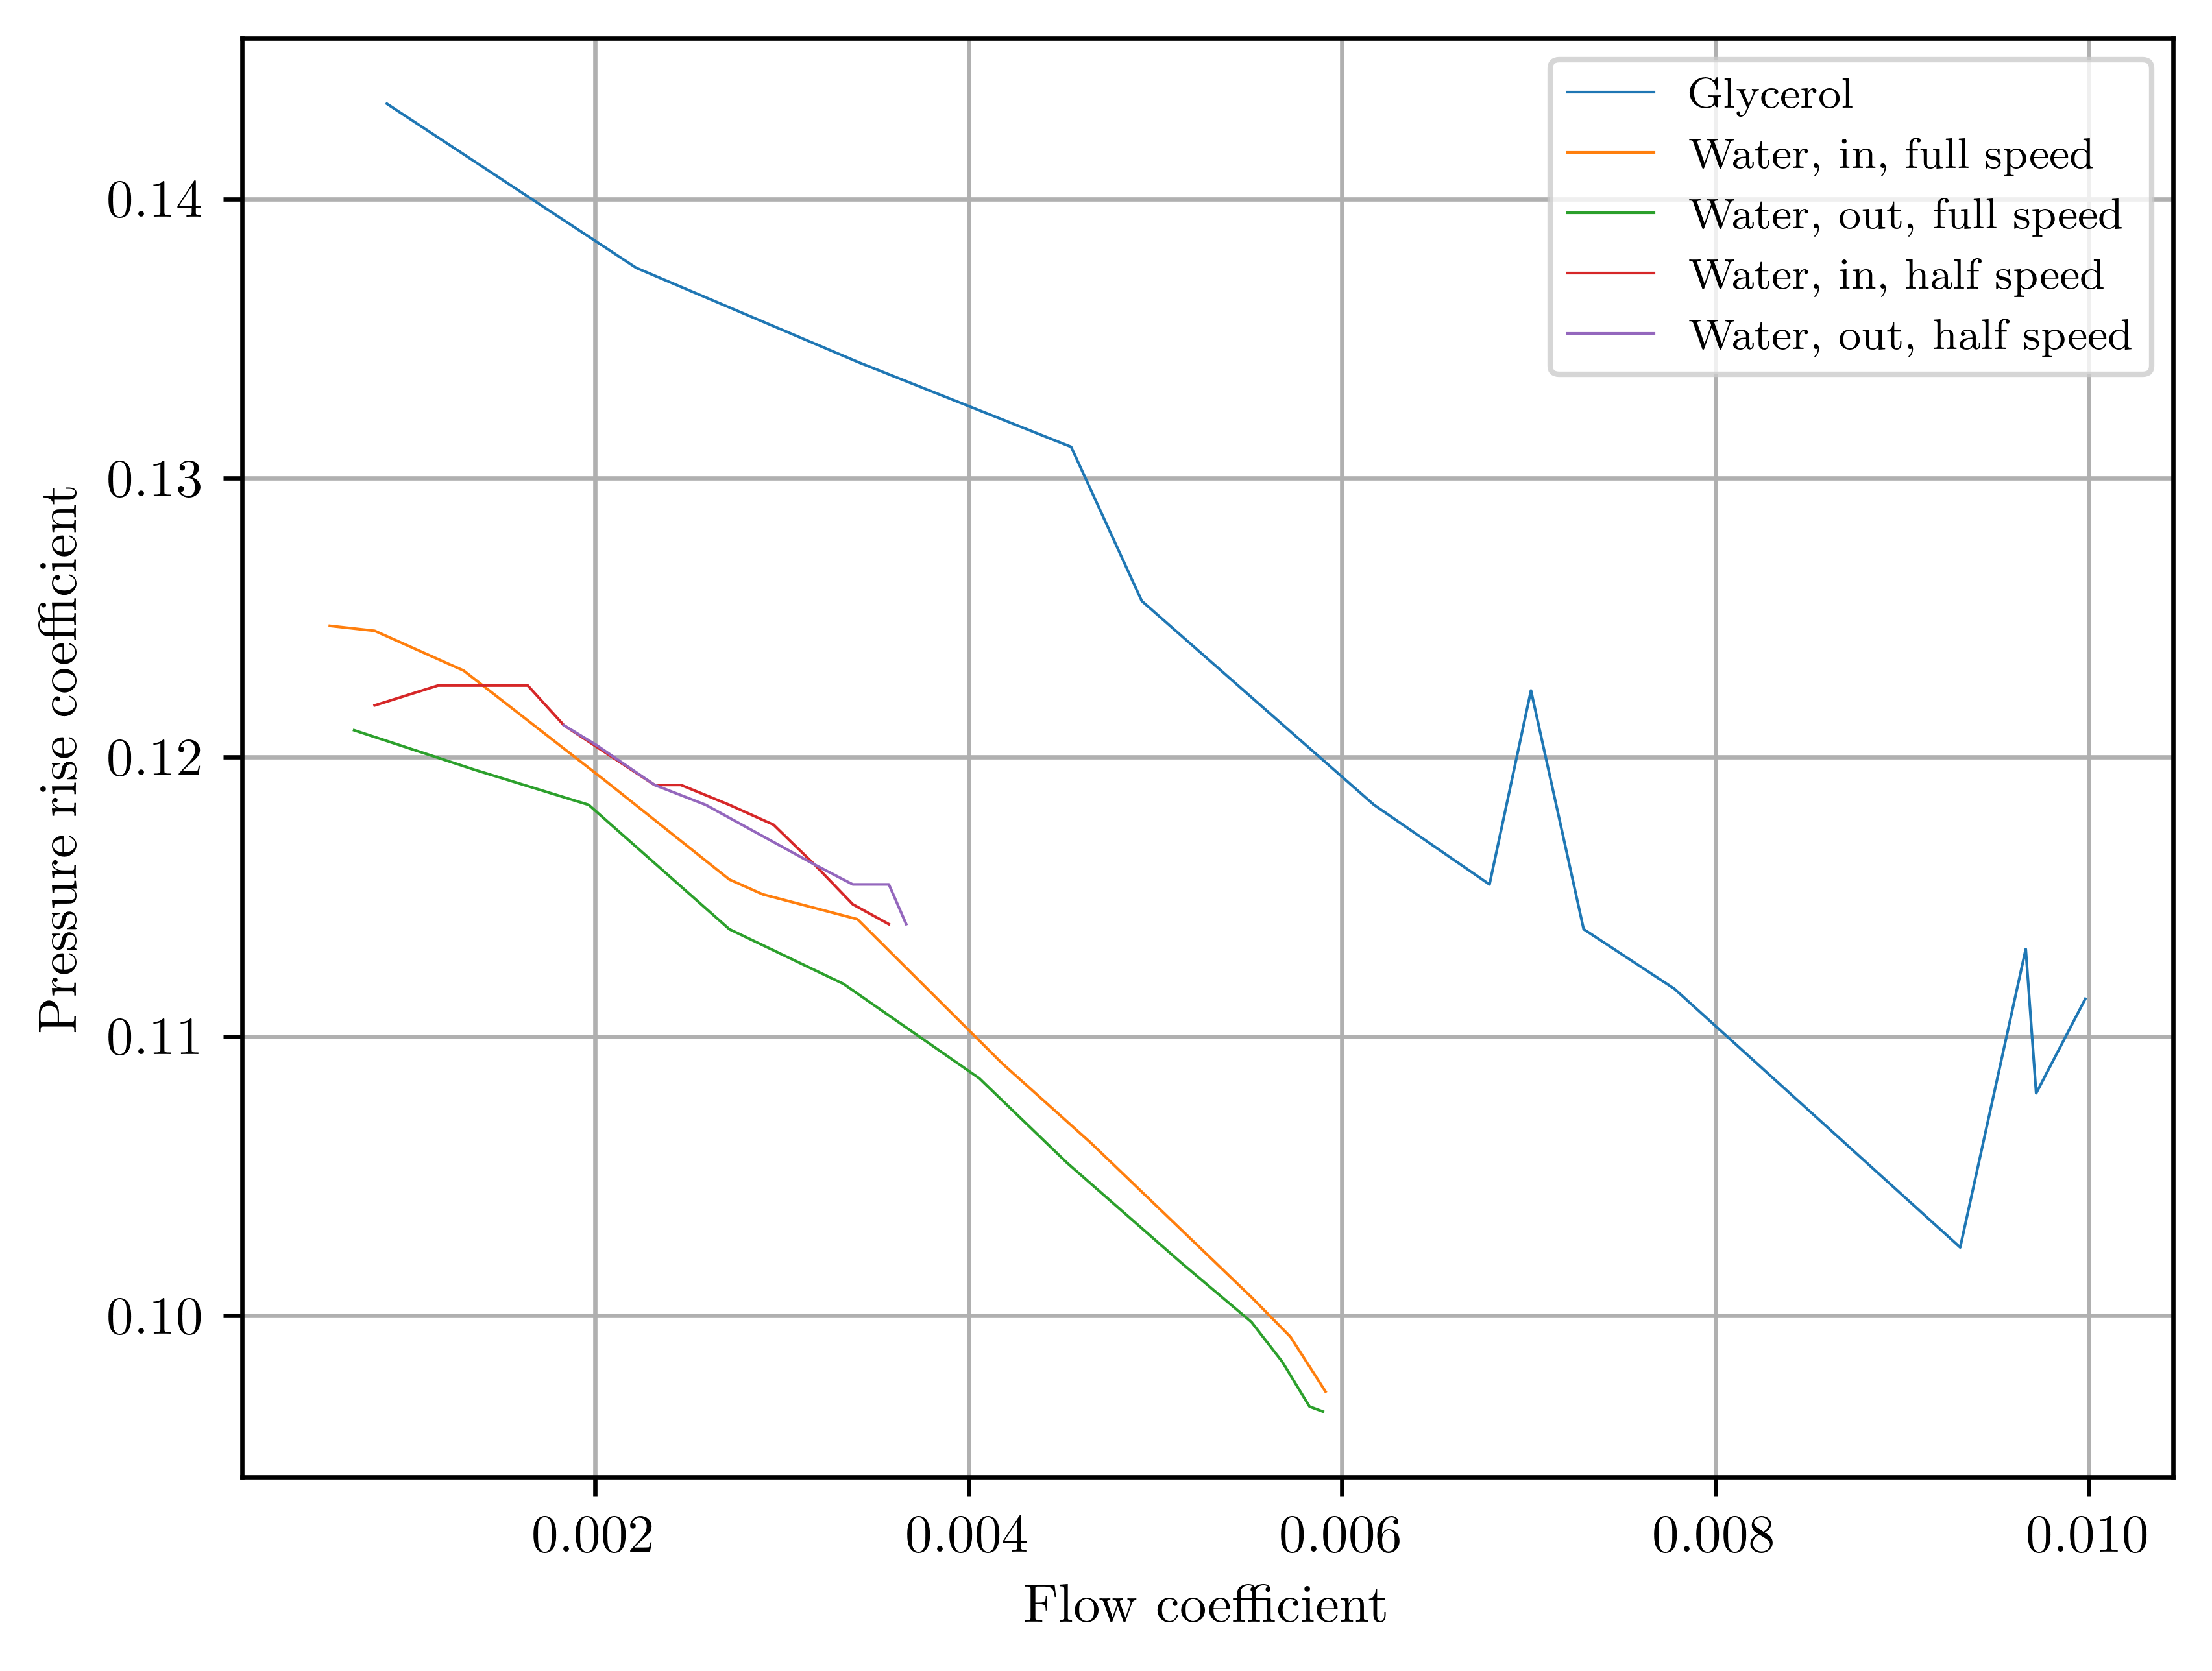
\includegraphics[width=0.9\textwidth]{compressor_non_dims.png}
    \caption{Non-dimensional pressure rise coefficient against non-dimensional flow coefficient various compressors conditions and setups.}
    \label{fig:compressor_non_dims}
\end{figure}

\begin{figure}[H]
    \centering
    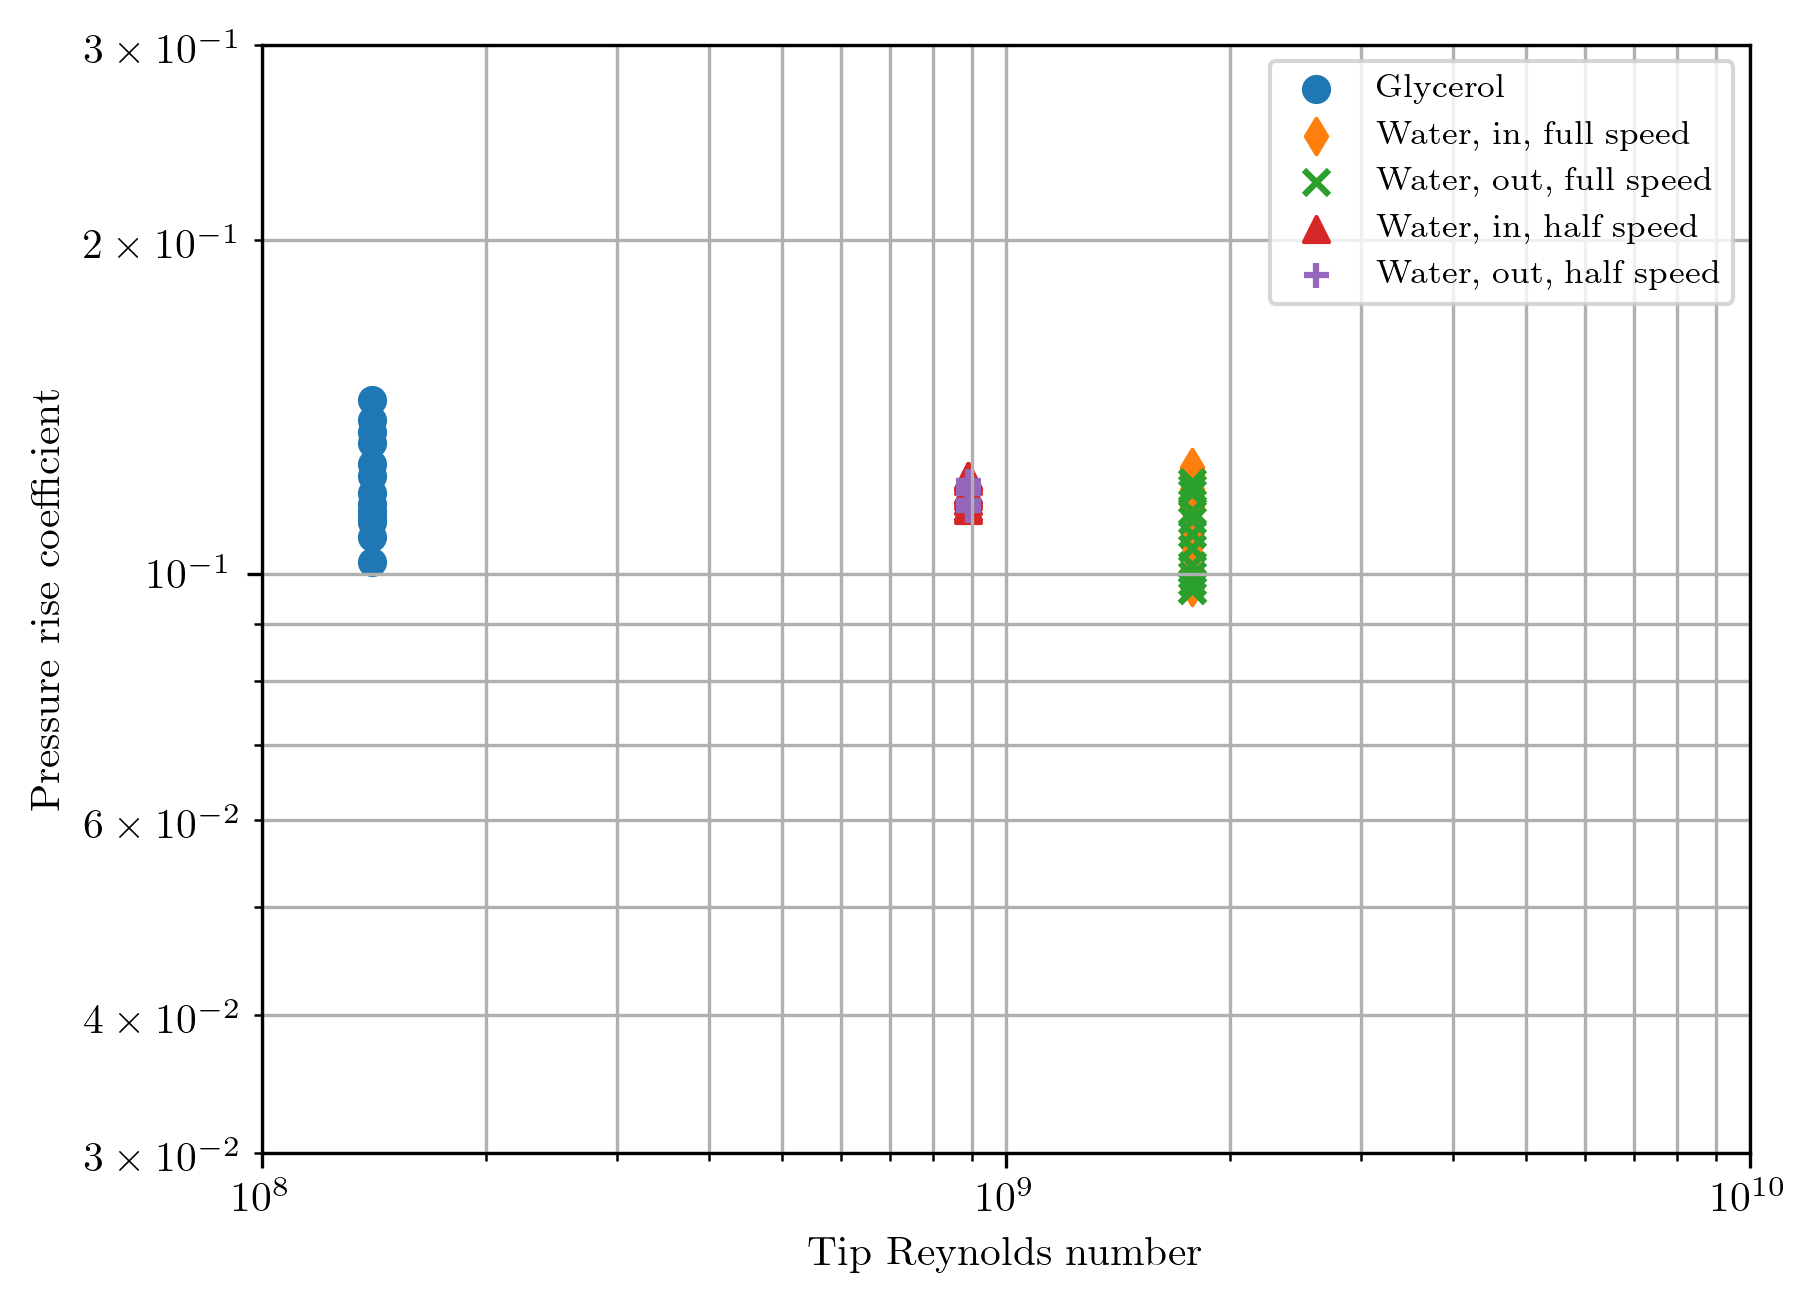
\includegraphics[width=0.9\textwidth]{pressure_reynolds.png}
    \caption{Pressure coefficient against tip Reynolds number for various compressor arrangements.}
    \label{fig:compressor_pressure_re}
\end{figure}

% Pressure Rise Coefficient against Tip Reynolds number.

\section{Discussion}
% Analyze and interpret the results, discussing their significance and any observations or trends.
% Do the results agree with what you expect for:
%% Change of pressure rise with flow rate

Figure \ref{fig:compressor_non_dims} shows that for all compressor arrangements, the pressure coefficient decrease with increasing flow coefficient.
This was expected for water from theory shown by the inverse relationship in equation \ref{eq:inverse_relationship}.
However, the gradient of the curves appears to initially increase, and then remains constant.
This was not expected, and is likely due to the compressor power increasing to maintain the same speed as the flow rate increases.
The isentropic efficiency of the compressor will also decrease at higher flow rates.

The area of the compressor channel increases, and so by continuity the velocity must decrease.
From Bernoulli's equation, this means that the pressure must increase in the radial direction.
The contribution of pressure on the torque of the compressor is the distance from the centre of the impeller multiplied by the circumferential component of pressure.
This may explain why impeller blades are curved, as to decrease this component of pressure further away from the centre of the impeller, reducing the torque and increasing efficiency.


% Explain why throttling the water compressor at inlet and exit produce different cavitation
% results. Also explain why the pressure rise is similar when cavitation is not present.

%% Change in cavitation with rotor speed and throttle location? Sketch two velocity
%% triangles, one at a nominal design condition and when the flow coefficient is much lower.

Cavitation was only observed for the smallest recorded flow rate while throttling inlet at the higher speed setting.
It was first detected visually using a stroboscope which was synchronised to the compressor speed.
It also occured at the smallest cavitation number, which shows that the cavitation number is a good predictor of cavitation.
Audible noise was also heard at lower inlet pressures where more severe cavitation was seen.
Cavitation bubbles were also observed to coalesce to form larger bubbles, which then collapsed.
This suggests that more severe caviation was occuring at the lower inlet pressures.

Cavitation was not observed for varying the outlet valve because throttling the outlet valve increases the pressure at compressor outlet.
This means that the pressure at the inlet is also increased and so the minimum pressure is above the vapour pressure of water,
and so cavitation is not expected to occur.

The location of cavitation was observed to be on the pressure surface but appeared to be further from the inlet than expected.
This means that the lowest static pressure is not at the inlet, and is instead further downstream on the trailing edge.
A possible reason for this may be that the flow must accelerate around the corner of the leading edge (See figure \ref{fig:flow_scenario_velocity_diagrams}), and so the pressure is
lowest further downstream than at the section of minimum area between leading and trailing edges.

The impact of cavitation on compressor performance was difficult to observe, as only one point of cavitation was observed.
However, it can be seen that just before the point of cavitation, the pressure rise coefficient appears to be constant with flow coefficient.
This is due to compressible 

%% Change of pressure rise with Reynolds number. Reference to figure 3 may be useful -
%% k/d is comparable to the roughness height of the blade surface divided by the channel span

%$ Can you explain the differences? Note that the two compressors do not give exactly the same
%% pressure rise-flow rate characteristics, and so care must be taken in comparing the effect of
%% Reynolds number.

Figure \ref{fig:compressor_pressure_re} shows that the Reynolds number of the glycerol setup is much lower than that of water.
This was expected due to its higher viscosity.


% Change in cavitation with rotor speed and throttle location? Sketch two velocity
% triangles, one at a nominal design condition and when the flow coefficient is much lower

\begin{figure}[H]
    \centering
    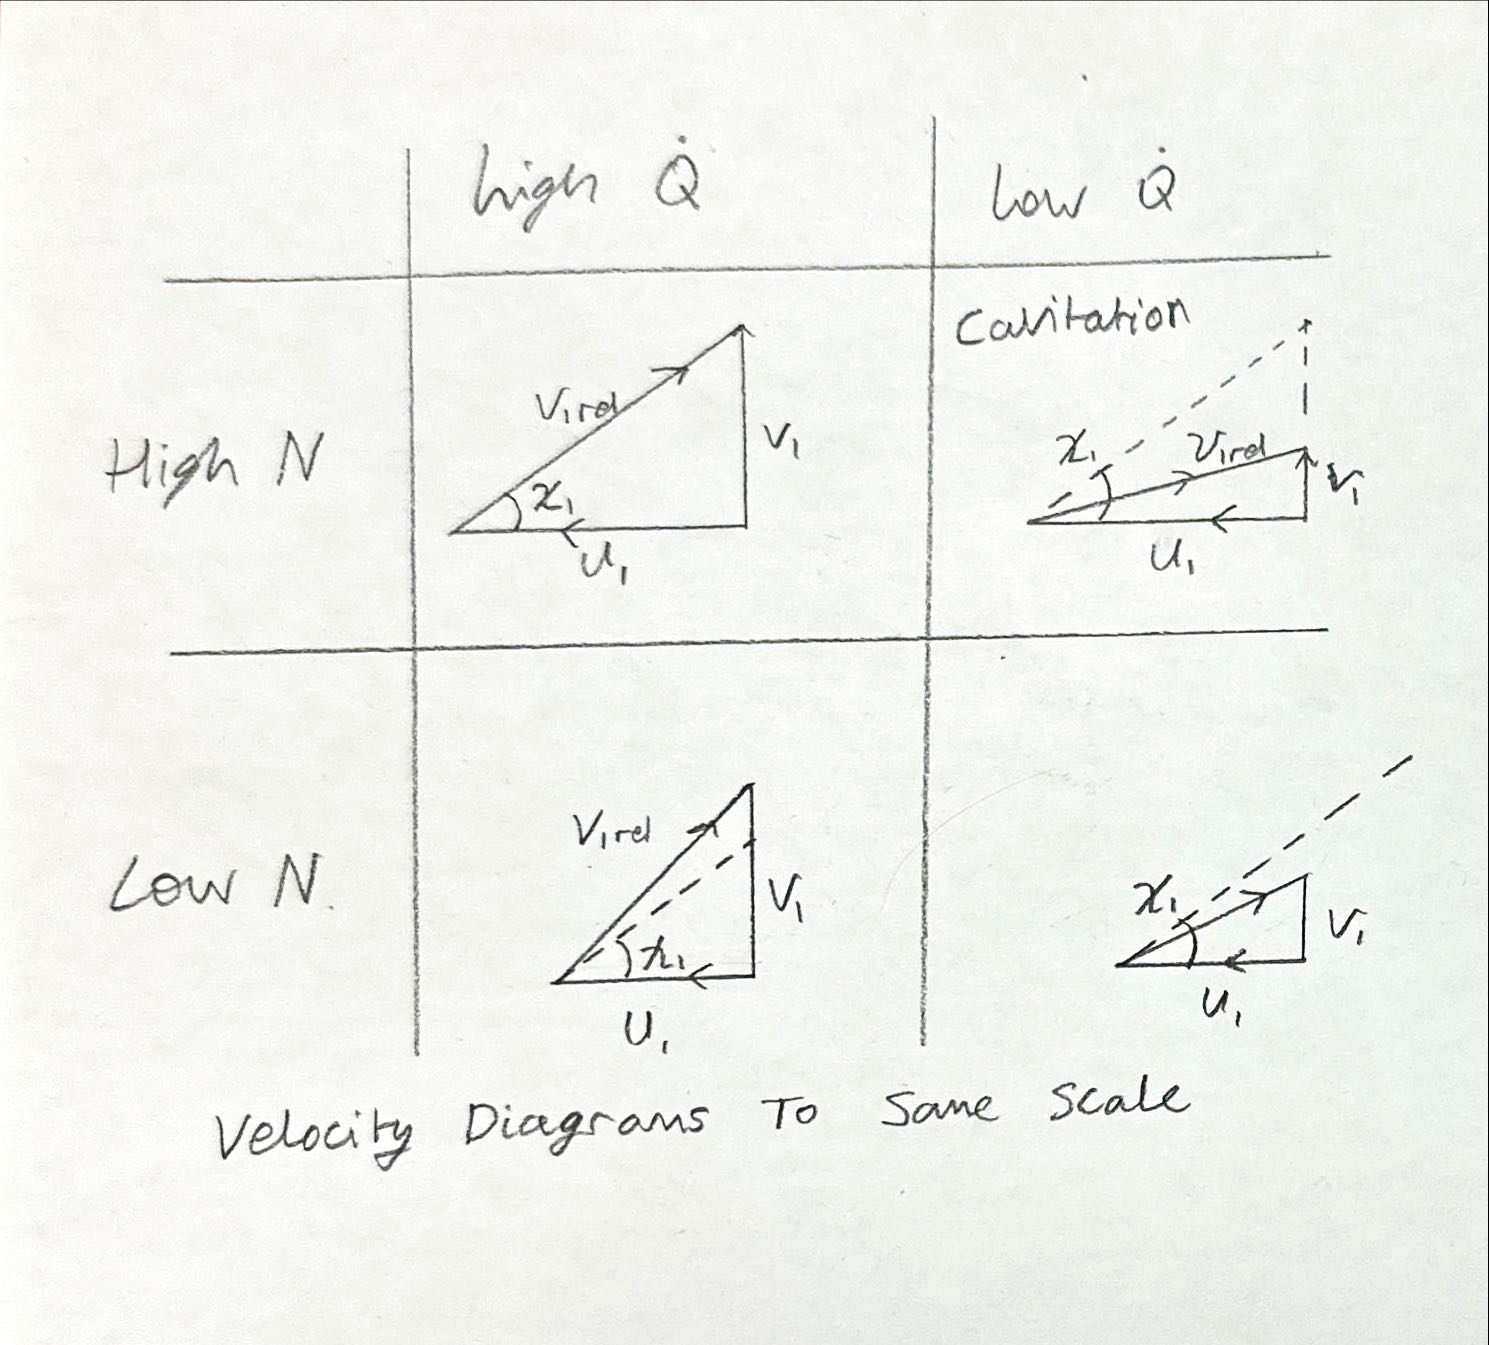
\includegraphics[width=0.6\textwidth]{flow_scenario_velocity_diagrams.jpg}
    \caption{Velocity diagrams for the compressor at nominal design condition and when the flow coefficient is much lower. The dashed line indicates the angle of blade leading edge.}
    \label{fig:flow_scenario_velocity_diagrams}
\end{figure}

The velocity diagrams for low flow and low speed are shown in figure \ref{fig:flow_scenario_velocity_diagrams}.
When compared to nominal design conditions at both high speed and high flow, the relative velocity is initially not aligned with the blade angle.
This means that the flow must turn to align with the blade angle.

% Suggest a reason why the venturi might not be suitable for measuring the flow rate of the
% glycerine solution.
The venturi flume may not be suitable for measuring flows of high viscosity fluids, as equation for mass flow rate \ref{eq:venturi_flume} 
is derived from Bernoulli's equation which assumes invicid flow.

\section{Conclusion}
% Summarize the main findings of the experiment and draw conclusions based on the results.

In conclusion, five compressor arrangements were tested, and the pressure rise and flow coefficients were calculated and plotted.
The pressure rise coefficient was found to decrease with increasing flow coefficient, 
which was correctly predicted from theory derived with a constant energy assumption.
Incompressible and invicid flow assumptions were used to understand pressure and velocity changes in the radial direction.


\section{Appendix}

\begin{table}[H]
    \centering
    \begin{tabular}{cccc}
        \hline
        Venturi Pressure (kPa) & Mass Flow (kg/s) & Compressor Pressure Rise (kPa) & Temperature ($^\circ C$)\\
        \hline
        20.7 & 0.8781 & 54.2 & 17.9 \\
        20.2 & 0.8674 & 54.3 & 17.9 \\
        19.2 & 0.8457 & 55.2 & 17.9 \\
        18.1 & 0.8211 & 56.0 & 17.9 \\
        15.7 & 0.7647 & 57.2 & 17.9 \\
        12.2 & 0.6741 & 59.2 & 17.9 \\
        9.8 & 0.6042 & 60.9 & 17.9 \\
        6.6 & 0.4958 & 62.8 & 17.9 \\
        4.4 & 0.4048 & 63.9 & 17.9 \\
        2.3 & 0.2927 & 66.4 & 17.9 \\
        1.1 & 0.2024 & 67.1 & 17.9 \\
        0.3 & 0.1057 & 67.9 & 17.9 \\
        \hline
    \end{tabular}
    \caption{Water full speed data on varied outlet valve flow}
    \label{tab:water_full_speed_outlet_data}
\end{table}

\begin{table}[H]
    \centering
    \begin{tabular}{cccc}
        \hline
        Venturi Pressure (kPa) & Mass Flow (kg/s) & Compressor Pressure Rise (kPa) & Temperature ($^\circ C$)\\        \hline
        2.0 & 0.2730 & 16 & 18.1 \\
        1.9 & 0.2660 & 16.2 & 18.2 \\
        1.7 & 0.2516 & 16.2 & 18.2 \\
        1.5 & 0.2364 & 16.3 & 18.2 \\
        1.0 & 0.1930 & 16.6 & 18.2 \\
        0.8 & 0.1726 & 16.7 & 18.2 \\
        0.6 & 0.1495 & 16.9 & 18.2 \\
        0.5 & 0.1365 & 17 & 18.2 \\
        \hline
    \end{tabular}
    \caption{Water half speed data on varied outlet valve flow.}
    \label{tab:water_half_speed_outlet_data}
\end{table}

\begin{table}[H]
    \centering
    \begin{tabular}{cccc}
        \hline
        Venturi Pressure (kPa) & Mass Flow (kg/s) & Compressor Pressure Rise (kPa) & Temperature ($^\circ C$)\\        \hline
        20.8 & 0.8802 & 54.6 & 18.3 \\
        19.5 & 0.8523 & 55.7 & 18.3 \\
        18.1 & 0.8211 & 56.5 & 18.3 \\
        12.9 & 0.6932 & 59.6 & 18.3 \\
        10.4 & 0.6224 & 61.2 & 18.3 \\
        6.9 & 0.5070 & 64.1 & 18.3 \\
        5.0 & 0.4316 & 64.6 & 18.3 \\
        4.4 & 0.4048 & 64.9 & 18.3 \\
        2.5 & 0.3052 & 66.9 & 18.4 \\
        1.0 & 0.1930 & 69.1 & 18.4 \\
        0.4 & 0.1221 & 69.9 & 18.4 \\
        0.2 & 0.0863 & 70.0 & 18.5 \\
        \hline
    \end{tabular}
    \caption{Water full speed data for varied inlet valve.}
    \label{tab:water_full_speed_inlet_data}
\end{table}

\begin{table}[H]
    \centering
    \begin{tabular}{cccc}
        \hline
        Venturi Pressure (kPa) & Mass Flow (kg/s) & Compressor Pressure Rise (kPa) & Temperature ($^\circ C$)\\        \hline
        1.9 & 0.2660 & 16.0 & 18.5 \\
        1.7 & 0.2516 & 16.1 & 18.5 \\
        1.5 & 0.2364 & 16.3 & 18.5 \\
        1.3 & 0.2201 & 16.5 & 18.5 \\
        1.1 & 0.2024 & 16.6 & 18.5 \\
        0.9 & 0.1831 & 16.7 & 18.5 \\
        0.8 & 0.1726 & 16.7 & 18.5 \\
        0.5 & 0.1365 & 17.0 & 18.5 \\
        0.4 & 0.1221 & 17.2 & 18.5 \\
        0.3 & 0.1057 & 17.2 & 18.5 \\
        0.2 & 0.0863 & 17.2 & 18.5 \\
        0.1 & 0.0610 & 17.1 & 18.5 \\
        \hline
    \end{tabular}
    \caption{Water half speed data for varied inlet valve.}
    \label{tab:water_half_speed_inlet_data}
\end{table}


\begin{table}[H]
    \centering
    \begin{tabular}{ccc}
        \hline
        Time (s)& Flow Rate (kg/s) & Pressure (kPa) \\
        \hline
        12.66 & 1.3862 & 57.5 \\
        12.13 & 1.4468 & 60.6 \\
        11.81 & 1.4860 & 62.5 \\
        12.2  & 1.4385  & 63.5 \\
        16.81 & 1.0440 & 68.7 \\
        25.91 & 0.6773 & 73.6 \\
        133.19 & 0.1318 & 80.5 \\
        53.09 & 0.3306 & 77.2 \\
        19.1  & 0.9188 & 66.4 \\
        16.16 & 1.0860 & 63.9 \\
        15.15 & 1.1584 & 62.7 \\
        34.55 & 0.5079 & 75.3 \\
        23.92 & 0.7336 & 70.5 \\
        17.36 & 1.0109   & 64.8 \\
        \hline
    \end{tabular}
    \caption{glycerine compressor data for varied outlet valve.}
    \label{tab:glycerine_outlet_data}
\end{table}


\begin{figure}[H]
    \centering
    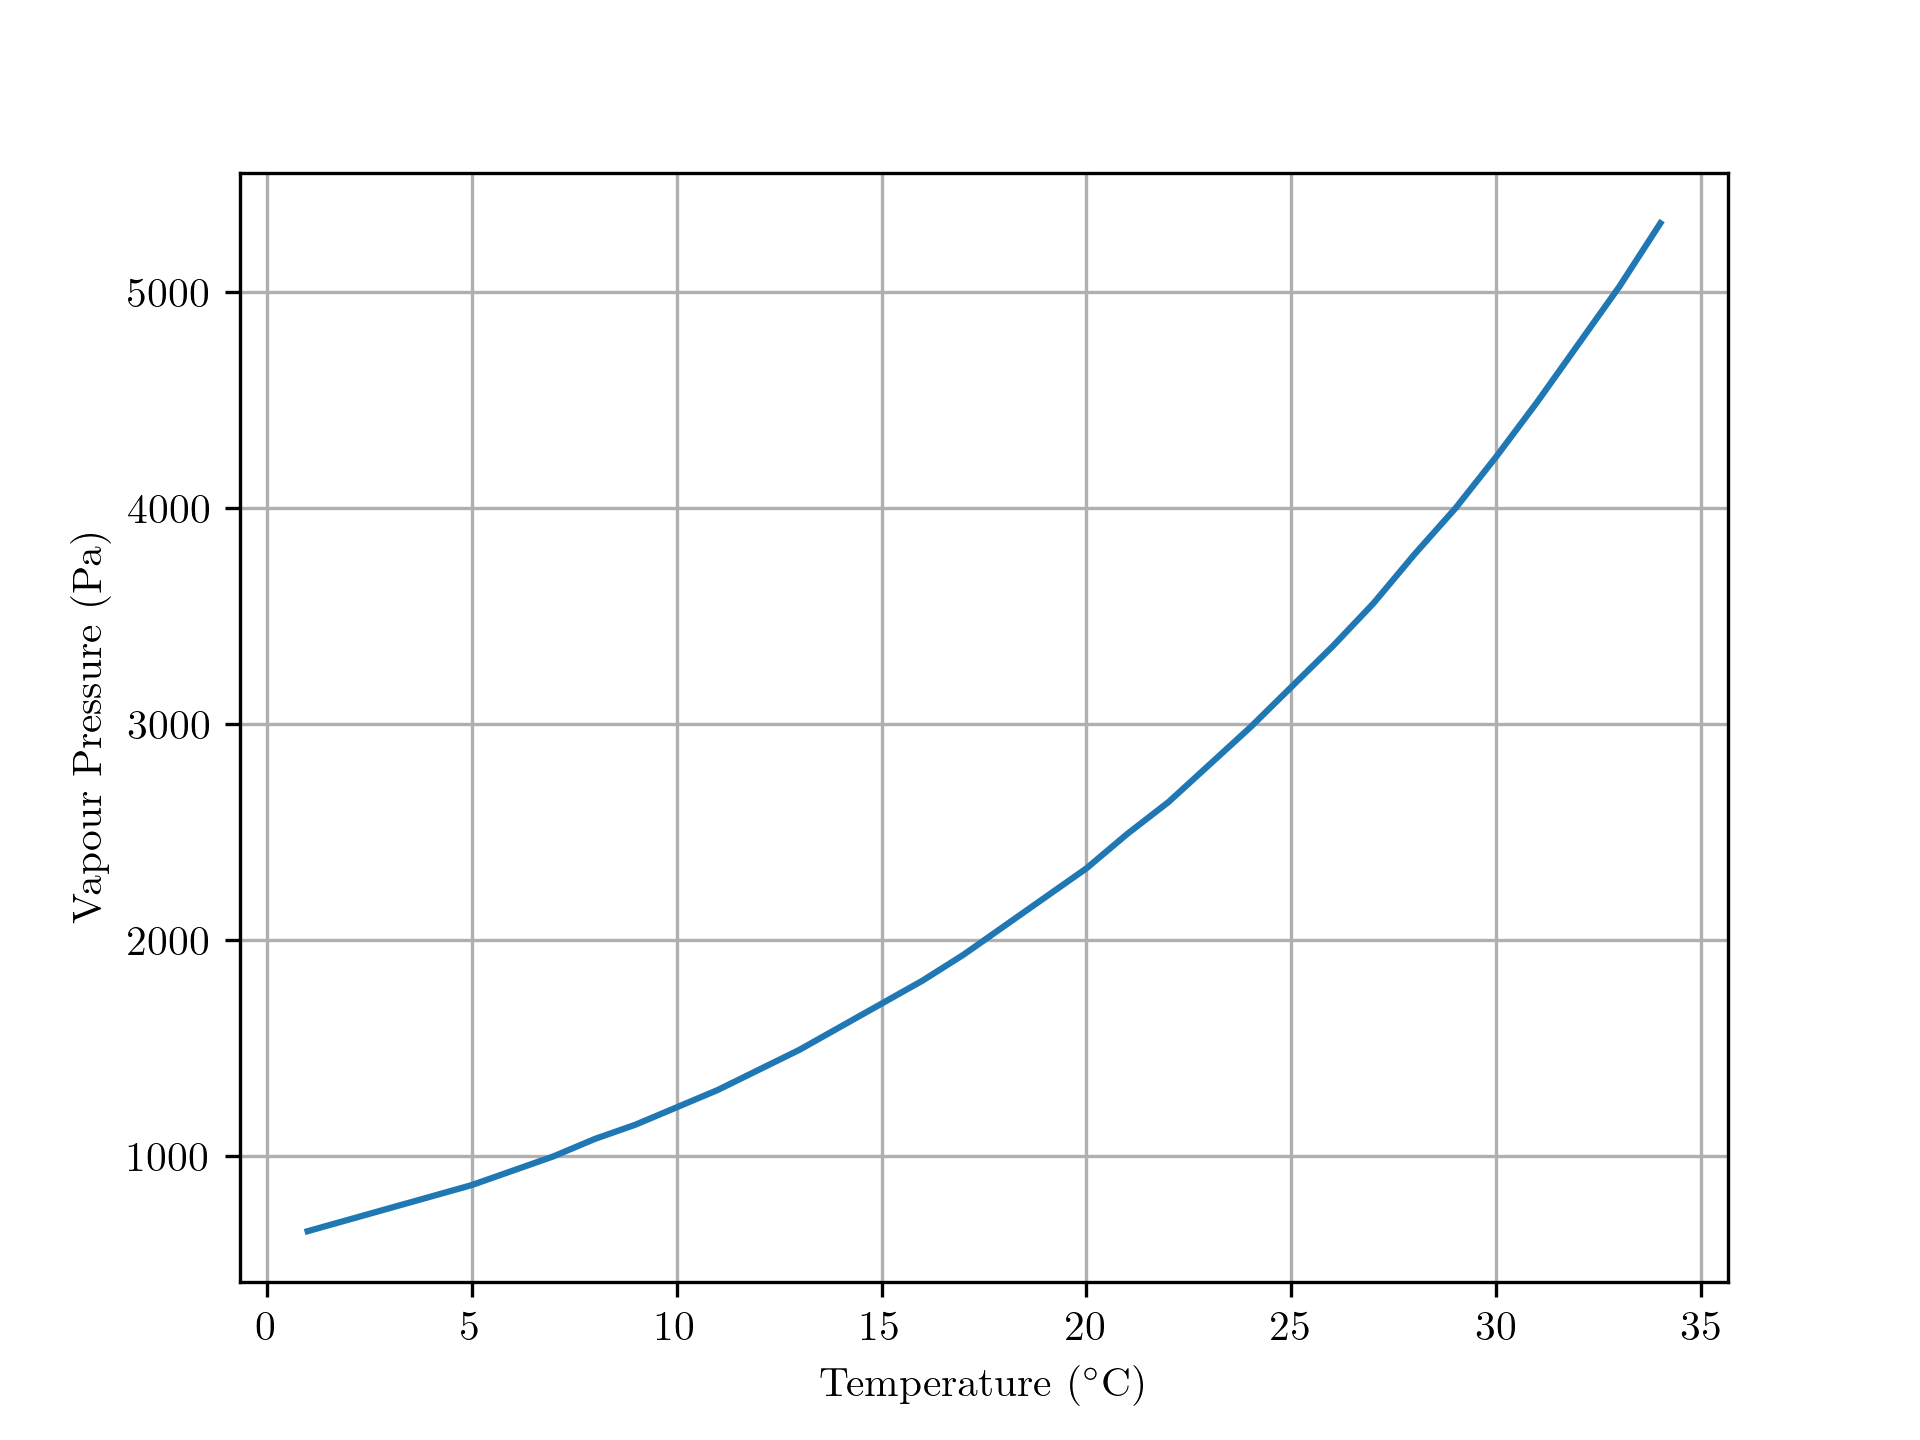
\includegraphics[width=0.9\textwidth]{vapour_pressure_water.png}
    \caption{Vapour pressure of water at various temperatures \cite{vapour_pressure}}
    \label{fig:vapour_pressure_water}
\end{figure}

\begin{figure}[H]
    \centering
    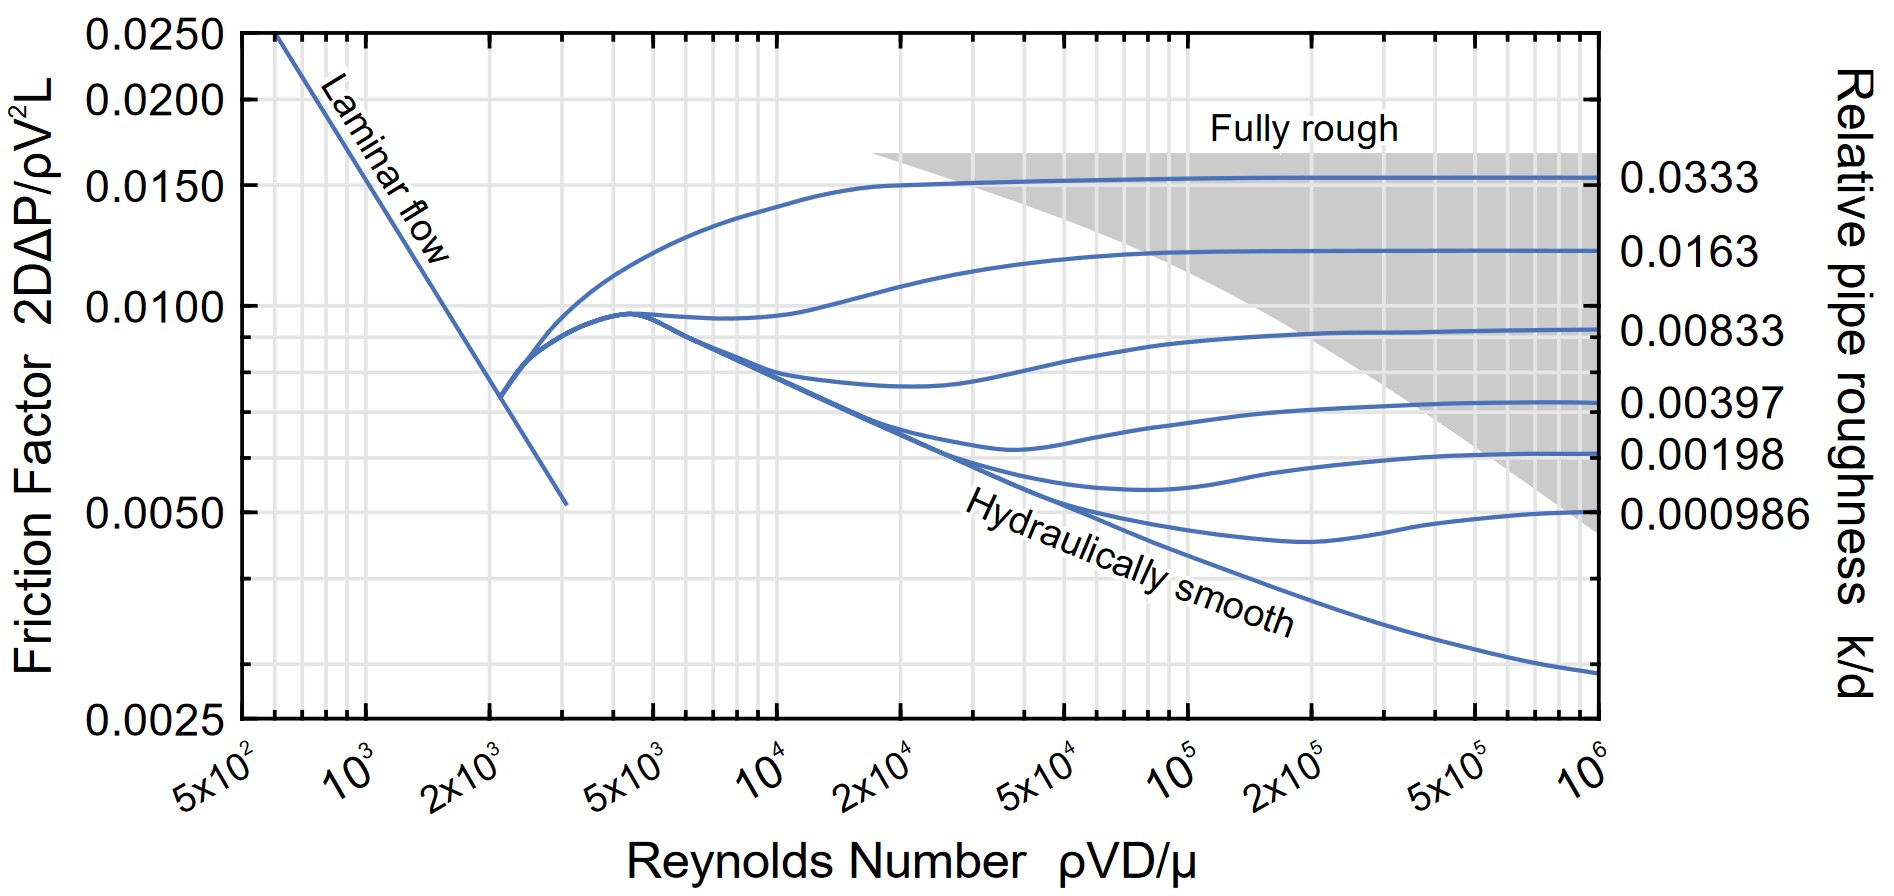
\includegraphics[width=0.9\textwidth]{re_roughness.jpg}
    \caption{Fricton factor vs Reynolds number for pipes of varying roughness \cite{handout}}
    \label{fig:Re_vs_friction_factor}
\end{figure}

\begin{thebibliography}{9}
    \bibitem{vapour_pressure} % help add link https://www.wiredchemist.com/chemistry/data/vapor-pressure
    The Wired Chemist ,\textit{Vapour Pressure of Water}, \texttt{https://www.wiredchemist.com/chemistry/data/vapor-pressure}, Accessed 2023.2.27
    \bibitem{handout}
    Taylor, J.V. 2023, \textit{Module 3A3: Radial Compressor Lab handout}
\end{thebibliography}

\end{document}
